% ============================================================================
%  Chapter 2 — DevSecOps Fundamentals and State of the Art
% ============================================================================

\chapter{DevSecOps Fundamentals and State of the Art}
\label{chap:fundamentals}

\section{Introduction}

Before getting into the technical details of our system, it is important to understand the concepts and technologies it is built on. In this chapter, we introduce the DevOps philosophy and how it evolved into DevSecOps, explain the shift-left security approach, cover the main Infrastructure as Code technologies, define what Policy-as-Code means, describe the design patterns we used, and finish with a comparison of existing security scanning tools.


% ────────────────────────────────────────────────────────────────────────────
\section{From DevOps to DevSecOps}
\label{sec:devops-devsecops}

\subsection{DevOps: Definition and Principles}

DevOps is a combination of practices, tools, and cultural ideas that bring together software development (\emph{Dev}) and IT operations (\emph{Ops}). The goal is to shorten the development cycle while delivering features and updates with better quality and speed~\cite{bass2015devops}. The main principles of DevOps are:

\begin{itemize}[leftmargin=1.5cm]
  \item \textbf{Continuous Integration (CI)}: Developers regularly merge their code into a shared repository, where automated builds and tests check that everything works.
  \item \textbf{Continuous Delivery/Deployment (CD)}: Once the code passes all checks, it is automatically prepared for release to production, with little or no manual work.
  \item \textbf{Infrastructure as Code}: Infrastructure is set up and managed through configuration files instead of manual steps.
  \item \textbf{Monitoring and Feedback}: Production systems are continuously monitored, and the data collected helps the team improve.
\end{itemize}

\begin{figure}[H]
\centering
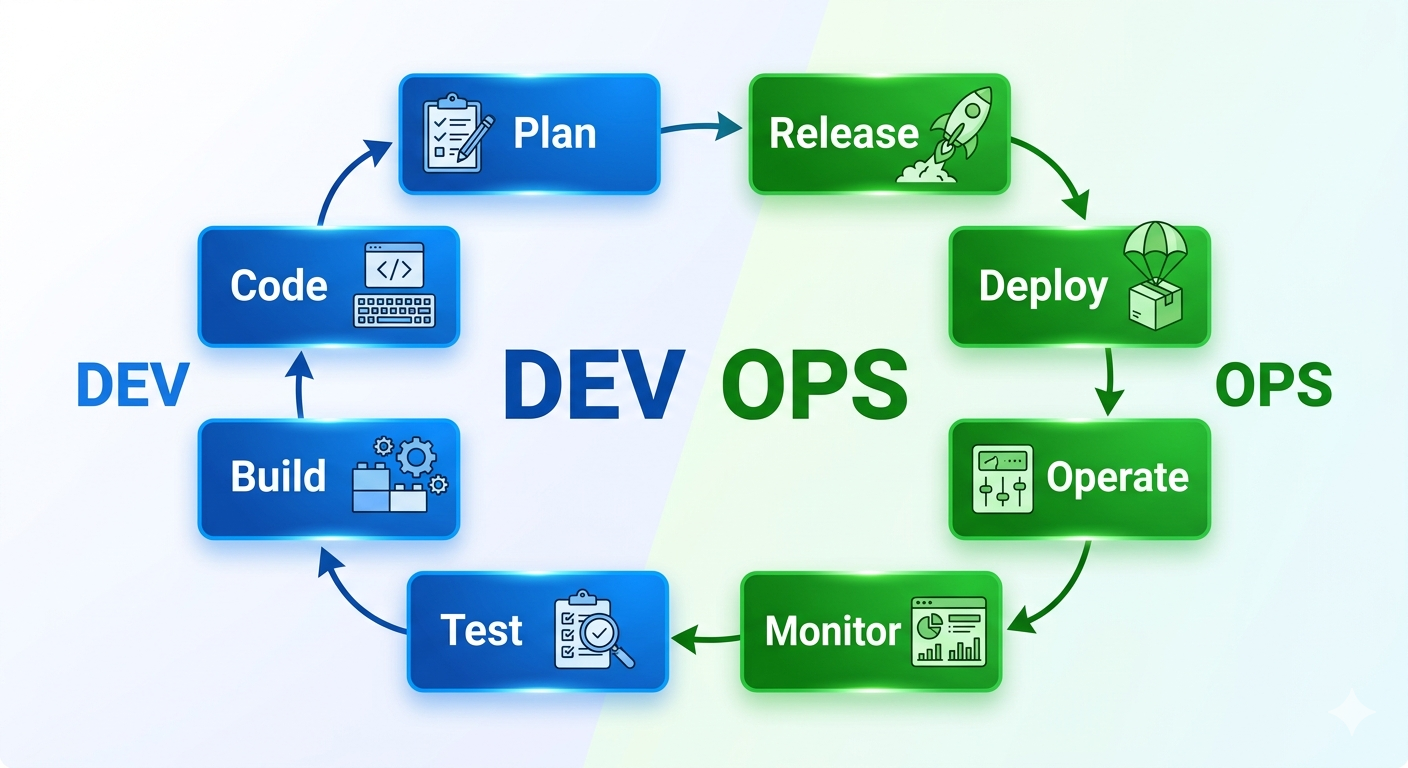
\includegraphics[width=0.80\textwidth]{images/DevOps.png}
\caption{The DevOps lifecycle: an iterative loop connecting development and operations stages.}
\label{fig:devops_lifecycle}
\end{figure}

\subsection{The Security Gap in Traditional DevOps}

While DevOps makes delivery much faster, it often treats security as a final checkpoint --- something done by a separate team right before release. This ``bolt-on'' approach creates several issues~\cite{rajapakse2022challenges}:

\begin{enumerate}[leftmargin=1.5cm]
  \item \textbf{Late discovery}: Finding a security problem during a pre-release review means going back and reworking code that was written weeks earlier, which is costly.
  \item \textbf{Bottleneck}: A single security team reviewing all changes becomes a constraint on how fast the team can deliver.
  \item \textbf{Cultural friction}: Developers start seeing security as an obstacle instead of a help, and they may try to work around it.
\end{enumerate}

\subsection{DevSecOps: Security as a Shared Responsibility}

DevSecOps extends DevOps by making security part of every stage of the development process. Instead of a single security phase at the end, automated checks are embedded at multiple points~\cite{myrbakken2017devsecops}:

\begin{itemize}[leftmargin=1.5cm]
  \item \textbf{At coding time}: IDE extensions flag insecure patterns while the developer is writing code.
  \item \textbf{At commit time}: Pre-commit hooks scan for secrets and misconfigurations.
  \item \textbf{At build time}: CI pipelines run static analysis and policy checks on infrastructure files.
  \item \textbf{At runtime}: Monitoring tools watch for unusual behavior and configuration changes.
\end{itemize}

\begin{figure}[H]
\centering
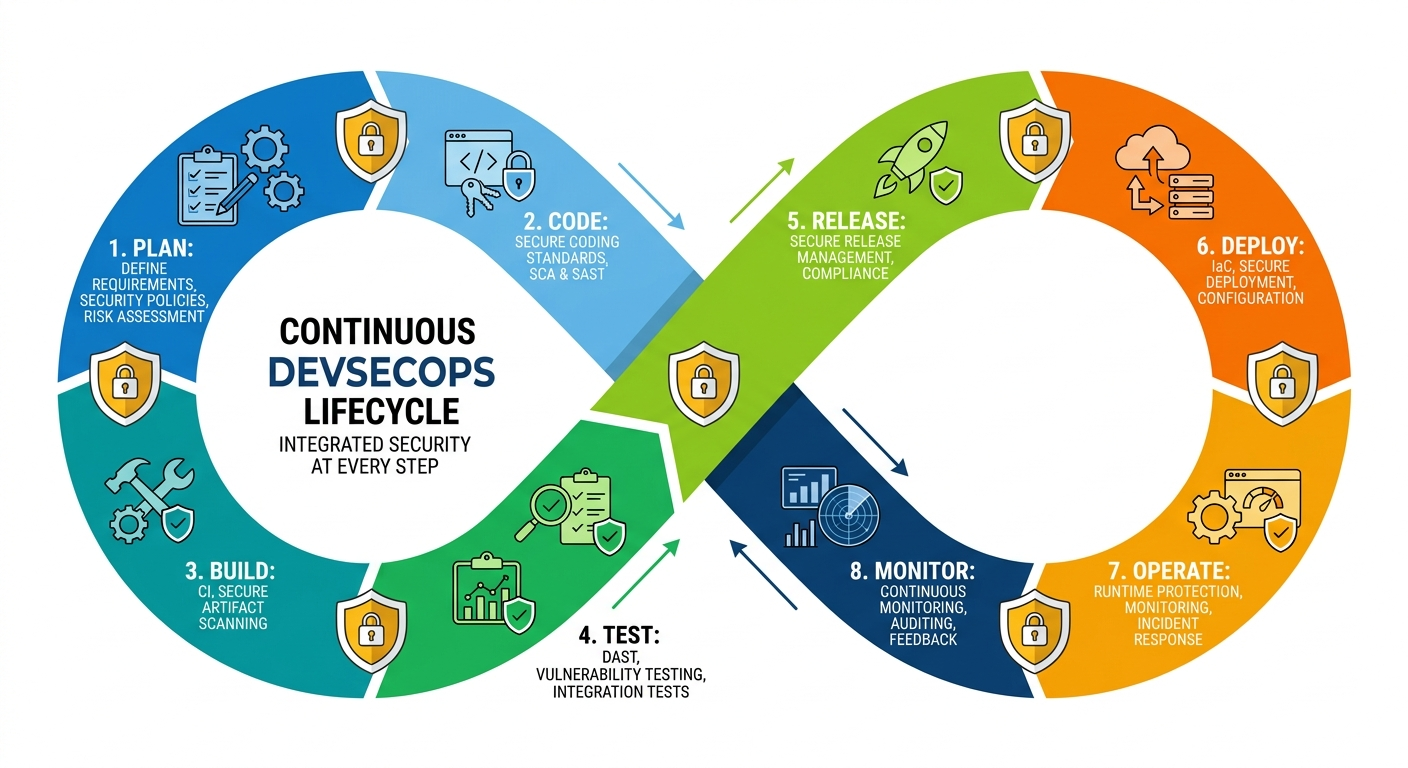
\includegraphics[width=0.80\textwidth]{images/DevSecOps.png}
\caption{The DevSecOps lifecycle: security is integrated at every stage of the development and operations loop.}
\label{fig:devsecops_lifecycle}
\end{figure}


% ────────────────────────────────────────────────────────────────────────────
\section{The Shift-Left Security Paradigm}
\label{sec:shiftleft}

The term \emph{shift-left} means moving quality and security checks earlier in the development process~\cite{mohan2016shiftleft}. For infrastructure security, this means catching misconfigurations at the moment the developer writes the IaC file, not after deployment when fixing things is much harder and more expensive.

The logic behind shift-left is simple: a bug found during coding is cheap to fix. The same bug found in production could mean downtime, data leaks, or compliance violations --- all of which cost much more.

Our microservice applies shift-left at three levels:

\begin{enumerate}[leftmargin=1.5cm]
  \item \textbf{IDE level}: The VS Code extension scans every time the developer saves a file, giving feedback in under a second with colored markers right in the editor.
  \item \textbf{Dashboard level}: The web interface lets developers scan and fix code interactively before committing it.
  \item \textbf{Pipeline level}: Jenkins integration acts as a last line of defense, blocking deployments that still have unresolved violations.
\end{enumerate}

\begin{figure}[H]
\centering
\begin{tikzpicture}[scale=0.95]
% Axes
\draw[-{Stealth}, thick] (0,0) -- (12,0) node[right] {\small\textbf{Time}};
\draw[-{Stealth}, thick] (0,0) -- (0,6) node[above] {\small\textbf{Cost to Fix}};

% Traditional approach (red curve)
\draw[very thick, color=red!70!black, smooth]
    plot coordinates {(1,0.3) (3,0.8) (5,1.5) (7,2.5) (9,4) (11,5.5)};
\node[color=red!70!black, font=\small\bfseries, anchor=west] at (9.5,5.8) {Traditional};

% Shift-left approach (green curve)
\draw[very thick, color=green!60!black, smooth]
    plot coordinates {(1,0.3) (3,0.5) (5,0.7) (7,0.9) (9,1.1) (11,1.3)};
\node[color=green!60!black, font=\small\bfseries, anchor=west] at (9.5,1.6) {Shift-Left};

% Phase labels on x-axis
\foreach \x/\lbl in {1.5/Code, 3.5/Build, 5.5/Test, 7.5/Release, 9.5/Prod} {
    \draw (\x, -0.1) -- (\x, 0.1);
    \node[font=\scriptsize, below] at (\x, -0.15) {\lbl};
}

% Savings annotation
\draw[{Stealth}-{Stealth}, thick, color=blue!60!black] (9, 1.1) -- (9, 4);
\node[font=\scriptsize\bfseries, color=blue!60!black, anchor=west] at (9.1, 2.55) {Savings};

\end{tikzpicture}
\caption{Shift-left security: finding and fixing defects earlier in the lifecycle costs significantly less.}
\label{fig:shiftleft}
\end{figure}


% ────────────────────────────────────────────────────────────────────────────
\section{Infrastructure as Code}
\label{sec:iac}

Infrastructure as Code (IaC) is the practice of managing computing infrastructure through machine-readable files instead of manual configuration~\cite{morris2020iac}. This approach brings the benefits of version control, peer review, automated testing, and reproducible environments to infrastructure management.

\subsection{Terraform}

Terraform, created by HashiCorp, is a declarative IaC tool that uses the HashiCorp Configuration Language (HCL) to define cloud resources across multiple providers like AWS, Azure, and GCP~\cite{hashicorp2024terraform}. You describe the desired state of your infrastructure, and Terraform figures out what changes to make to get there.

\begin{lstlisting}[language=terraform, caption={Example Terraform resource definition for an AWS S3 bucket.}, label={lst:terraform-example}]
resource "aws_s3_bucket" "data_store" {
  bucket = "company-data-store"
  acl    = "private"
  
  server_side_encryption_configuration {
    rule {
      apply_server_side_encryption_by_default {
        sse_algorithm = "AES256"
      }
    }
  }
  
  tags = {
    Environment = "production"
    Owner       = "platform-team"
  }
}
\end{lstlisting}

\subsection{Docker}

Docker allows you to package applications and their dependencies into lightweight, portable containers~\cite{docker2024docs, turnbull2014docker}. A \texttt{Dockerfile} defines the steps to build a container image: the base image, installed packages, configuration settings, and the command to run.

\begin{lstlisting}[language=dockerfile, caption={Example Dockerfile with security best practices.}, label={lst:dockerfile-example}]
FROM python:3.10-slim

WORKDIR /app
COPY requirements.txt .
RUN pip install --no-cache-dir -r requirements.txt
COPY . .

RUN useradd -m -u 1000 appuser
USER appuser

HEALTHCHECK --interval=30s --timeout=3s CMD curl -f http://localhost:8000/health || exit 1

CMD ["python", "main.py"]
\end{lstlisting}

\subsection{Kubernetes}

Kubernetes is an open-source platform that automates the deployment, scaling, and management of containerized applications~\cite{kubernetes2024docs, burns2022kubernetes}. Resources in Kubernetes are defined using YAML files that describe the desired state of pods, deployments, services, and other objects.

\begin{lstlisting}[language=yaml, caption={Example Kubernetes Deployment manifest.}, label={lst:k8s-example}]
apiVersion: apps/v1
kind: Deployment
metadata:
  name: web-app
spec:
  replicas: 3
  template:
    spec:
      containers:
        - name: app
          image: myapp:1.2.0
          securityContext:
            privileged: false
            runAsUser: 1000
          resources:
            limits:
              cpu: "500m"
              memory: "256Mi"
\end{lstlisting}


% ────────────────────────────────────────────────────────────────────────────
\section{Policy-as-Code}
\label{sec:policy-as-code}

Policy-as-Code is an approach where security and compliance rules are written as executable code instead of plain text documents~\cite{openpolicyagent2024}. This offers several advantages over traditional policy management:

\begin{itemize}[leftmargin=1.5cm]
  \item \textbf{Consistency}: Policies are applied the same way every time, removing subjective interpretation.
  \item \textbf{Auditability}: Policy definitions are version-controlled, so there is always a clear record of what was enforced and when.
  \item \textbf{Automation}: Policies can be checked automatically inside CI/CD pipelines, without needing a human to review them.
  \item \textbf{Extensibility}: New policies can be added easily as new threats or compliance requirements come up.
\end{itemize}

In our microservice, each of the 103~policies is implemented as a Python class with a standard \texttt{check()} method. This makes the system both easy to extend and easy to test. Policies are organized into 15~categories covering cloud services (AWS S3, EC2, RDS, IAM, VPC), container security (Docker, Kubernetes), and general infrastructure best practices (logging, tagging, encryption).


% ────────────────────────────────────────────────────────────────────────────
\section{Design Patterns}
\label{sec:patterns}

The architecture of our microservice uses several well-known software design patterns~\cite{gamma1994patterns, martin2017cleanarch} to keep things modular, maintainable, and easy to extend:

\begin{table}[H]
\centering
\begin{tabularx}{\textwidth}{|l|l|X|}
\hline
\textbf{Pattern} & \textbf{Component} & \textbf{How We Used It} \\
\hline
Strategy & Parser Layer & Different parser implementations (\texttt{TerraformParser}, \texttt{DockerfileParser}, \texttt{KubernetesParser}) are selected at runtime based on the input file type. \\
\hline
Template Method & Policy Engine & \texttt{BasePolicy} defines an abstract \texttt{check()} method; each concrete policy class overrides it with its own logic while sharing the same interface. \\
\hline
Factory & Parser Selection & The \texttt{get\_parser()} function acts as a factory that returns the right parser based on the \texttt{code\_type} parameter. \\
\hline
Layered Architecture & Global System & The four-layer design (API $\rightarrow$ Parser $\rightarrow$ Normalizer $\rightarrow$ Policy Engine) separates concerns and keeps dependencies flowing in one direction. \\
\hline
Observer & VS Code Extension & The extension listens for the \texttt{onDidSaveTextDocument} event and automatically triggers a scan whenever the developer saves a file. \\
\hline
\end{tabularx}
\caption{Design patterns used in the microservice.}
\label{tab:design-patterns}
\end{table}


% ────────────────────────────────────────────────────────────────────────────
\section{Comparative Study of Existing Tools}
\label{sec:comparative}

Several open-source tools exist for infrastructure security scanning. Table~\ref{tab:tool-comparison} compares our service with the four most widely used alternatives.

\begin{table}[H]
\centering
\begin{tabular}{|l|c|c|c|c|c|}
\hline
\textbf{Feature} & \textbf{Our Service} & \textbf{Checkov}~\cite{bridgecrew2024checkov} & \textbf{tfsec}~\cite{aquasecurity2024tfsec} & \textbf{Trivy}~\cite{aquasecurity2024trivy} & \textbf{OPA}~\cite{openpolicyagent2024} \\
\hline
Avg.\ response time    & \textbf{46\,ms} & 150--300\,ms & $\sim$150\,ms & $\sim$200\,ms & Varies \\
\hline
Auto-fix engine       & \textbf{Yes}    & No           & No            & No            & No     \\
\hline
VS Code extension     & \textbf{Yes}    & No           & No            & No            & No     \\
\hline
Web dashboard         & \textbf{Yes}    & No           & No            & No            & No     \\
\hline
Prometheus/Grafana    & \textbf{Yes}    & No           & No            & No            & No     \\
\hline
Educational feedback  & \textbf{Yes}    & Partial      & No            & No            & No     \\
\hline
Severity threshold    & \textbf{Yes}    & No           & No            & No            & No     \\
\hline
Fully offline         & \textbf{Yes}    & Yes          & Yes           & Yes           & No     \\
\hline
Multi-format support  & 3 formats       & 20+ formats  & Terraform     & Multi         & Any    \\
\hline
Community size        & Academic        & Large        & Large         & Large         & Large  \\
\hline
\end{tabular}
\caption{Comparison of infrastructure security scanning tools.}
\label{tab:tool-comparison}
\end{table}

\subsection{Analysis}

\textbf{Checkov}~\cite{bridgecrew2024checkov}, developed by Bridgecrew (now part of Palo Alto Networks), is the most feature-rich open-source scanner. It supports over 20 frameworks and has thousands of built-in checks. However, it only works from the command line --- there is no graphical interface, no auto-fix, and no built-in monitoring or IDE integration.

\textbf{tfsec}~\cite{aquasecurity2024tfsec}, by Aqua Security, focuses only on Terraform and offers fast, targeted scanning. Its main limitation is that it only supports one format and has no remediation features.

\textbf{Trivy}~\cite{aquasecurity2024trivy}, also by Aqua Security, started as a container vulnerability scanner and has grown to cover IaC, container images, and software dependencies. While it is powerful, it lacks interactive features like dashboards and automatic code fixing.

\textbf{Open Policy Agent (OPA)}~\cite{openpolicyagent2024} takes a different approach entirely. It is a general-purpose policy engine that uses its own Rego language. While very flexible, OPA requires significant expertise to write and maintain policies and depends on external infrastructure to run.

\vspace{0.3cm}
\noindent What makes our service different is that it \textbf{combines} six capabilities that no single existing tool offers together: fast API-based scanning, automatic code fixing, real-time IDE integration, an interactive web dashboard, configurable severity thresholds with educational feedback, and built-in Prometheus/Grafana monitoring --- all in a fully offline, self-contained package.


% ────────────────────────────────────────────────────────────────────────────
\section{Conclusion}

This chapter covered the theoretical and technical foundation for the project. We traced the evolution from DevOps to DevSecOps, explained the shift-left security approach, surveyed the three IaC technologies our service supports, defined Policy-as-Code, listed the design patterns we used, and compared our solution with existing tools. The next chapter presents the requirements analysis, system architecture, and sprint planning.
